\documentclass[12pt,a4paper,oneside]{report}

% MAC F312 self-study project report. Compile with pdfLaTeX.
\usepackage[margin=1in]{geometry}
\usepackage[T1]{fontenc}
% lmodern unavailable in sandbox
\usepackage[expansion=false]{microtype}
\usepackage{setspace}
\usepackage{graphicx}
\usepackage{booktabs}
\usepackage{tabularx}
\usepackage{array}
\usepackage{float}
\usepackage{amsmath,amssymb}
\usepackage{enumitem}
\usepackage{xcolor}
\usepackage[hidelinks]{hyperref}
\usepackage[nameinlink,noabbrev]{cleveref}

\linespread{1.12}\selectfont
\setlength{\parindent}{0pt}
\setlength{\parskip}{0.55em}
\renewcommand{\arraystretch}{1.18}
\setlength{\emergencystretch}{3em}
\graphicspath{{./}{./figures/}{C:/Users/sarth/sign-language-recognition/sign-language-recognition/report/figures/}}

\newcommand{\course}{MAC F312: Foundations of Data Science}
\newcommand{\projecttitle}{Isolated Sign Language Recognition Using Pose Estimation and Machine Learning: A WLASL-100 Study}
\newcommand{\studentone}{Sarthak Shrivastava}
\newcommand{\studenttwo}{Sahil Singh Chauhan}
\newcommand{\institution}{Birla Institute of Technology and Science, Pilani}
\newcommand{\reportdate}{4 November 2026}
\newcommand{\submissiondate}{4 November 2026}
\newcommand{\studentoneid}{2024ADPS0740P}
\newcommand{\studenttwoid}{2024ADPS0650P}
\newcommand{\discipline}{B.E. Mathematics and Computing}
\newcommand{\instructor}{Dr Niladri Chatterjee}

\begin{document}

% ---------- Cover (PS1 report style) ----------
\begin{titlepage}
\centering
\vspace*{0.4cm}
{\bfseries A REPORT\par}
\vspace{0.5em}
{\bfseries ON\par}
\vspace{0.5em}
{\bfseries ISOLATED SIGN LANGUAGE RECOGNITION USING\\ POSE ESTIMATION AND MACHINE LEARNING:\\ A WLASL-100 STUDY\par}
\vspace{1.6cm}
BY\par
\vspace{1.2cm}
\begin{flushleft}
\hspace*{0.3cm}\begin{tabular}{@{}p{4cm}p{3.2cm}p{6.5cm}@{}}
Name of the student & ID No. & Discipline \\
\studentone & \studentoneid & \discipline \\
\studenttwo & \studenttwoid & \discipline \\
\end{tabular}
\end{flushleft}
\vspace{1.2cm}
{\bfseries Prepared in complete fulfillment of the\\ Self-Study Project component of\\ \course\par}
\vspace{0.7cm}
{\bfseries Submitted to\par}
\vspace{0.25cm}
{\bfseries Dr Niladri Chatterjee\par}
Department of Mathematics\par
BITS Pilani\par
\vspace{0.5cm}

\includegraphics[width=2.6cm]{bits_logo.png}\par
\vspace{0.5cm}
{\bfseries BIRLA INSTITUTE OF TECHNOLOGY \& SCIENCE, PILANI\par}
\vspace{0.6em}
{\bfseries \reportdate\par}
\end{titlepage}

% ---------- Information page ----------
\thispagestyle{empty}
\begin{center}
{\bfseries BIRLA INSTITUTE OF TECHNOLOGY \& SCIENCE, PILANI}\\
{\bfseries Department of Mathematics}
\end{center}
\vspace{0.3em}
\setlength{\parskip}{0.45em}
\noindent\textbf{Course:} \course\par\vspace{0.25em}
\noindent\textbf{Date of submission:} \submissiondate\par\vspace{0.25em}
\noindent\textbf{Title of the project:} \projecttitle\par\vspace{0.25em}
\noindent\textbf{Students:} \studentoneid, \studentone, \discipline; \studenttwoid, \studenttwo, \discipline\par\vspace{0.25em}
\noindent\textbf{Course instructor:} \instructor, Department of Mathematics\par\vspace{0.25em}
\noindent\textbf{Key words:} sign language recognition, WLASL-100, MediaPipe Holistic, landmark features, signer-independent evaluation, classification\par\vspace{0.25em}
\noindent\textbf{Project area(s):} Data Science and Machine Learning\par\vspace{0.45em}
\noindent\textbf{Abstract:} We built a landmark-based classifier for isolated ASL signs using the WLASL-100 subset. Of its 2,038 listed clips, 1,466 were available for this study: 1,013 from a Kaggle mirror and 453 from the repository. MediaPipe Holistic landmarks were extracted for each clip, and the data were split by signer into 868 training, 294 validation, and 304 test clips. We compared six classical classifiers and two recurrent models, selecting settings with signer-grouped cross-validation. Extra Trees had the highest test accuracy (61.8\%), followed by logistic regression (60.5\%). These scores come from a single held-out group of signers. The limited video recovery, missing hand detections, and small number of clips for many glosses remain important limits on the results.

\setlength{\parskip}{0.55em}

% ---------- Acknowledgements ----------
\clearpage
\pagenumbering{roman}
\setcounter{page}{3}
\chapter*{Acknowledgements}
We would like to thank Dr Niladri Chatterjee, Department of Mathematics, for giving us the opportunity to undertake this self-study project as part of \course. The project gave us the scope to explore isolated sign language recognition as a practical application of data science and machine learning, and to work with a real video dataset rather than only with prepared examples.

Through this work, we were able to take part in the different stages of a machine-learning study: preparing and organizing the data, extracting pose landmarks from video, designing signer-independent experiments, comparing models, and interpreting their results. These steps helped us connect ideas from the course with the practical decisions and challenges involved in building an end-to-end project. We are grateful for the opportunity to pursue a topic that let us learn by working through these stages ourselves.

We also thank each other for the steady collaboration needed to assemble the videos, check the extracted landmarks, and work through the experiments. The WLASL dataset made this study possible, and we acknowledge its authors for providing a benchmark with signer metadata. We used open-source software throughout the project, including MediaPipe for landmark extraction, NumPy and pandas for data handling, scikit-learn and XGBoost for classical models, and PyTorch for the LSTM and GRU experiments. We are grateful to the maintainers of these tools and to the broader research community whose documentation helped us put the pipeline together.

\pagenumbering{roman}
\tableofcontents
\listoffigures
\listoftables
\clearpage
\pagenumbering{arabic}
\renewcommand{\thepage}{\arabic{page}}
\setcounter{page}{1}

\chapter{Introduction}
\section{Background}
Sign languages communicate through coordinated hand shape and motion, body posture, and facial or head cues. Recognizing an isolated sign from a short video is a multi-class classification task: a clip is assigned one word-level gloss. It differs from continuous sign-language translation, which must also locate sign boundaries and model sentence-level structure.

This project explores a lightweight recognition pipeline based on pose landmarks rather than raw video pixels. Landmark features reduce the visual input to body and hand coordinates and make it possible to compare classical machine-learning methods with temporal neural networks.

\section{Problem statement}
The objective is to classify each WLASL-100 video instance into one of 100 gloss classes while evaluating on signers absent from model training. The main methodological challenge is to build a reproducible pipeline despite incomplete video availability, missing landmarks, and substantial signer variation.

\section{Objectives}
\begin{enumerate}[leftmargin=*]
  \item Audit the WLASL-100 metadata and establish a reproducible, signer-independent dataset split.
  \item Obtain available clips and extract pose and hand landmarks once for downstream experiments.
  \item Quantify clip, signer, class, and landmark coverage before modelling.
  \item Compare coordinate, angle, velocity, and temporal aggregation choices.
  \item Tune classical and recurrent classifiers without signer leakage and report held-out test performance.
\end{enumerate}

\section{Questions guiding the experiments}
We organized the work around three practical questions. First, how much information about an isolated gloss can be recovered from body and hand landmarks alone? Second, which representation and model family performs best when signers in evaluation were not seen during training? Third, how much does a random clip split change the apparent result when signers overlap? These questions keep the analysis focused on the choices we could measure with the data available. They also shaped the experiments: channel ablations address the first question, grouped cross-validation and the frozen test split address the second, and the random-split diagnostic illustrates the third.

\section{Why signer independence matters}
An evaluation split should match the kind of generalization we want to measure. If the same people appear in both training and test data, a model can benefit from recurring recording conditions or signer-specific movement patterns. This is especially important for a relatively small dataset, where a model might learn the style of a few frequent signers rather than features that transfer to people it has not seen. We therefore treat signer identity as a grouping variable throughout the main evaluation, even though it is not an input feature for the classifiers.

\section{Scope}
We focus on recognizing one pre-segmented sign per clip from the WLASL-100 subset. We use MediaPipe Holistic landmarks rather than training directly on video pixels. Continuous signing, sentence translation, and a live-camera application are outside this project.

\chapter{Related Work}
\section{Word-level sign recognition}
Word-level sign recognition assigns a gloss to a pre-segmented sign video. The segmentation is assumed to be given: each example already contains one intended sign, so the model does not need to detect where a sign begins or ends. This makes the task narrower than continuous sign recognition, but still challenging because the same gloss can look different across people and recordings.

WLASL provides word-level ASL clips and signer metadata for benchmarking recognition across a large set of glosses. The dataset paper evaluates video-based recognition methods; we use the WLASL-100 subset for a landmark-based pipeline and focus on a signer-independent comparison \cite{li2020wlasl}. The subset gives us a fixed vocabulary of 100 glosses and enough signer variation to make the split strategy a central part of the experiment.

\section{Pose-based representations}
Pose estimation represents a person using a set of body joints. For sign recognition, hands carry detailed information about configuration and movement; upper-body landmarks add context and provide a reference for where the hands are positioned. A landmark representation can be smaller and easier to inspect than raw pixels, but it depends on the pose estimator returning stable points. Missed hands or inconsistent coordinates become missing or noisy model inputs.

MediaPipe Holistic estimates pose and hand landmarks in a unified pipeline \cite{mediapipe_holistic}. In this project, each frame contains 33 pose points and 21 points for each hand, with three coordinates per point, for 225 values per frame. We keep this representation rather than cropping each hand to an image because the project goal is to compare a shared set of geometric features across classical and temporal models.

\section{Classical and temporal classifiers}
We use classical classifiers as strong, relatively quick baselines for compact feature vectors. Logistic regression provides a linear decision boundary and a useful reference point. kNN assigns a class based on nearby training examples, so it depends on scaling and on the selected distance neighbourhood. An RBF SVM can describe nonlinear boundaries through a kernel. Random Forest and Extra Trees average many decision trees, while XGBoost builds trees sequentially to correct errors from previous trees. These models make different assumptions about the geometry of the input, which is why one representation need not suit all of them equally well.

LSTM and GRU networks instead read a sequence one frame at a time and maintain a hidden state. Both are gated recurrent models designed to retain information across a sequence. We use bidirectional versions so that the representation of a frame can incorporate information from both earlier and later frames in the clip. These models have more trainable parameters than the fixed-vector baselines and can overfit when the number of clips per class is small. The comparison is therefore useful even when the recurrent models do not lead the final scores.

The scikit-learn tools provide the classical pipelines and grouped cross-validation used here \cite{sklearn}. XGBoost supplies the gradient-boosted tree model, and PyTorch supplies the recurrent networks \cite{xgboost,pytorch}. In every case, a model's reported score depends on the representation, the fitting procedure, and the split; comparing algorithm names alone would not be meaningful.

\section{Evaluation and signer leakage}
Recordings from the same signer can share appearance, camera placement, clothing, and signing style. If clips from one signer appear in both training and test sets, a model may exploit signer-specific cues. We therefore keep signers disjoint across train, validation, and test partitions and use signer-grouped folds during model selection.

\chapter{Data and Methodology}
\section{Dataset and availability}
The WLASL-100 subset contains 2,038 metadata instances across 100 glosses. We kept the official WLASL-100 class list. Many original video links no longer worked, so we assembled the usable set from videos already in the repository and a Kaggle mirror. Landmark arrays are available for 1,466 clips: 1,013 from Kaggle and 453 from the repository. The remaining 572 instances could not be recovered and were excluded.

This recovery step determined the final size of every later experiment. We did not replace missing clips with duplicate instances or change the 100-class vocabulary to fit the recovered videos. Instead, the original metadata and frozen signer split remain the reference, and each experiment uses the clips for which landmarks were available. The collection has a median of 14.5 recovered clips per gloss, with a range from 9 to 23. This is a small number for a 100-class problem, and performance for individual glosses is sensitive to which clips fall in each partition.

\begin{table}[H]
\centering
\label{tab:data}
\begin{tabular}{lr}
\toprule
Source & Clips \\
\midrule
Kaggle mirror & 1,013 \\
Project repository & 453 \\
Total usable clips & 1,466 \\
Not available & 572 \\
Metadata total & 2,038 \\
\bottomrule
\end{tabular}
\caption{Available landmark clips used in the experiments.}
\end{table}

The clips are unevenly distributed across signers as well as glosses. There are 73 signers in the usable landmark set. The median signer contributes eight clips, but the largest signer contributes 243 clips, about one sixth of the entire collection. The split is signer-independent, so these clips stay together in a single partition. This prevents direct signer leakage, but it also means the number of videos in each partition is not a simple random 65/15/20 percent division. One large signer can make a partition noticeably larger and can influence the results for the glosses that signer performs.

\begin{table}[H]
\centering
\label{tab:class-support}
\begin{tabular}{lrrr}
\toprule
Summary & Minimum & Median & Maximum \\
\midrule
Recovered clips per gloss & 9 & 14.5 & 23 \\
Signers per gloss & 7 & 11 & 14 \\
Clips per signer & 1 & 8 & 243 \\
\bottomrule
\end{tabular}
\caption{Variation in clip and signer support across the available data.}
\end{table}

\section{Signer-independent partitions}
Our frozen split has 868 training, 294 validation, and 304 test clips. It includes 46, 12, and 15 signers in those partitions, with no signer appearing in more than one. The split configuration searched 2,000 seeded GroupShuffleSplit assignments, preferring coverage of all classes and at least two clips per class in validation and test. The chosen split uses seed 165. We then intersected those assignments with the available landmark IDs and used the same resulting split for each experiment.

All 100 glosses appear in each partition, but the desired minimum counts were not met for every class: 11 glosses have only one validation clip, two glosses have only one test clip, and ``tell'' has four training clips. We keep these cases rather than silently moving clips across signer boundaries. The trade-off is that macro-averaged and per-class metrics can be noisy for these rare cases. The split is fixed in \texttt{split\_v2.csv}; the assignment was not regenerated separately for each model.

\begin{table}[H]
\centering
\label{tab:split}
\begin{tabular}{lrrr}
\toprule
Partition & Clips & Signers & Classes \\
\midrule
Train & 868 & 46 & 100 \\
Validation & 294 & 12 & 100 \\
Test & 304 & 15 & 100 \\
\bottomrule
\end{tabular}
\caption{Frozen signer-independent split.}
\end{table}

\section{Landmark extraction and quality checks}
We ran MediaPipe Holistic once for each available video and saved one NumPy array per clip. Each frame has 33 body-pose points, 21 left-hand points, and 21 right-hand points, with $(x,y,z)$ coordinates, for 225 values in total. Missed detections are kept as missing values. We use the saved clip frame ranges; bounding-box cropping is off by default because the boxes for some YouTube-derived clips are unreliable.

We checked overlays for 20 clips against their video frames. The body pose usually follows the signer, but hand points are less reliable; some clips show only one hand clearly. The median clip length is 70 frames. Across clips, the median missing-coordinate rate is 31.6\%. Pose is detected in nearly every frame, while median hand missingness varies from about 38\% to 81\% depending on the source and hand.

The source-level summaries show the same pattern. Pose missingness is essentially zero at the median for both sources, but hand missingness is much higher. The Kaggle arrays have median missingness of about 67.9\% for the left hand and 41.8\% for the right hand. The repository arrays have median missingness of about 80.6\% for the left hand and 38.1\% for the right hand. These numbers are computed over the landmark points, not over the full clip count. They help explain why left-hand-only features perform poorly and why a missingness mask is useful for recurrent inputs.

\begin{table}[H]
\centering
\label{tab:missingness}
\begin{tabular}{lrrrr}
\toprule
Source & Clips & Median frames & Left hand missing & Right hand missing \\
\midrule
Kaggle & 1,013 & 65 & 67.9\% & 41.8\% \\
Repository & 453 & 77 & 80.6\% & 38.1\% \\
\bottomrule
\end{tabular}
\caption{Median per-point hand missingness by landmark source.}
\end{table}

\begin{figure}[H]
\centering
\IfFileExists{C:/Users/sarth/sign-language-recognition/sign-language-recognition/report/figures/landmark_overlay_sample.png}{\includegraphics[width=0.95\textwidth]{C:/Users/sarth/sign-language-recognition/sign-language-recognition/report/figures/landmark_overlay_sample.png}}{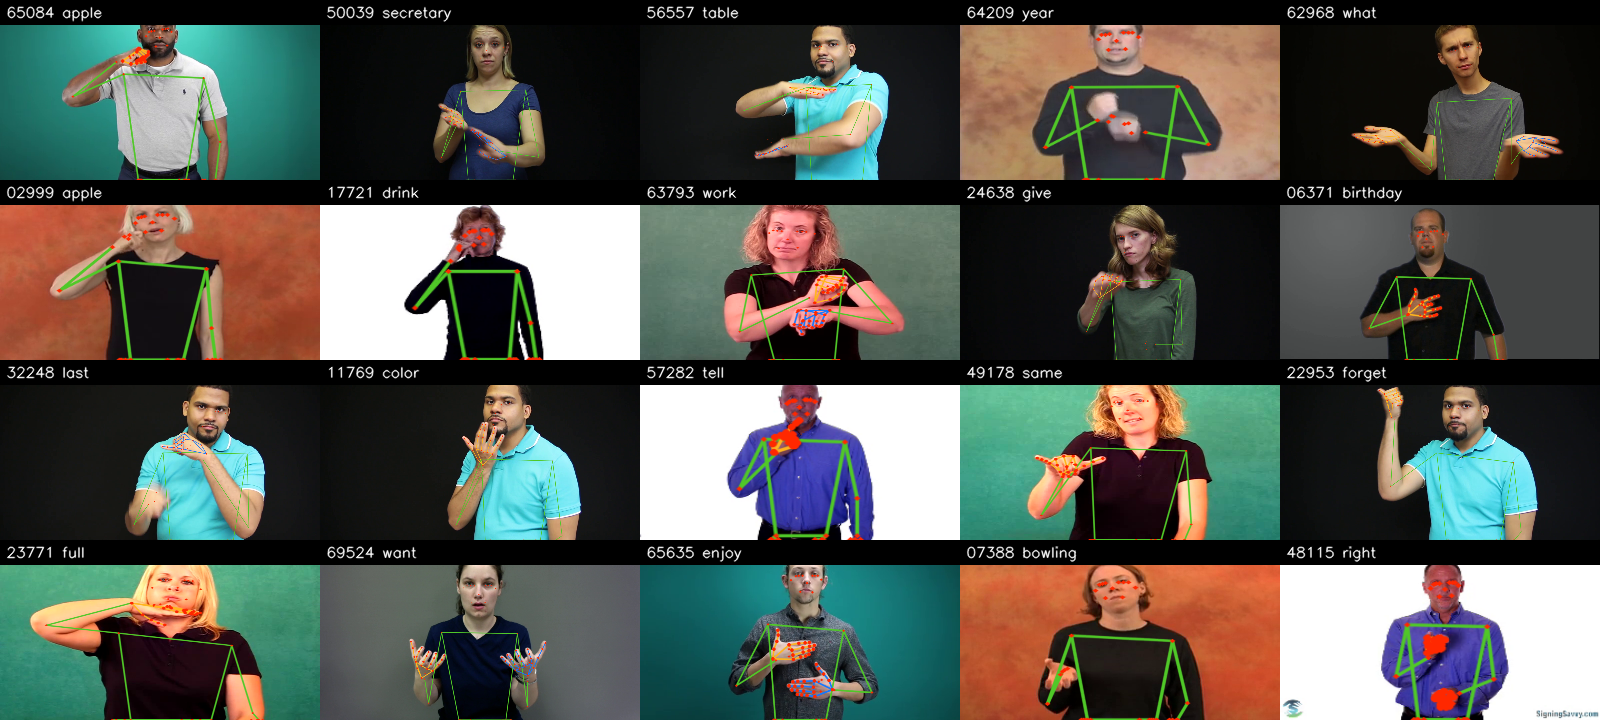
\includegraphics[width=0.95\textwidth]{landmark_overlay_sample.png}}
\caption{Sample visual quality check of extracted pose and hand landmarks.}
\label{fig:overlays}
\end{figure}

\section{Preprocessing and features}
We interpolate gaps of up to three frames and leave longer gaps missing. Coordinates are centered on the shoulders and scaled by shoulder width, then resampled to a fixed sequence length. The saved feature bundle contains normalized coordinates, frame-to-frame velocity, and joint angles. For the classical comparison, we summarize 64 frames in two temporal bins using both hands and their angles. For LSTM and GRU, we use 32-frame hand-and-angle sequences and provide a mask that marks missing values.

For a frame with shoulder locations $p_L$ and $p_R$, we define the shoulder centre as $c=(p_L+p_R)/2$ and the scale as $s=\lVert p_L-p_R\rVert_2$. A finite landmark coordinate $p$ is transformed to $(p-c)/s$. This reduces the effect of image translation and signer distance from the camera, while preserving a relative position with respect to the upper body. If shoulder width is missing or too close to zero, it is treated as missing rather than used as an unstable scale.

We calculate angular features from selected triples of landmarks. Given joint locations $a,b,c$, the angle at $b$ is
\[
\theta = \arccos\left(\frac{(a-b)\cdot(c-b)}{\lVert a-b\rVert_2\,\lVert c-b\rVert_2}\right).
\]
The feature set includes selected upper-body and hand-joint angles. Angles describe local configuration while being less sensitive than raw coordinates to overall movement across the frame. They are still affected by missed or noisy landmarks, so unavailable angles remain missing.

Velocity is approximated by the difference between consecutive resampled coordinates. It captures direction and magnitude of movement between frames but can also amplify landmark noise. This is one reason we treat velocity as an ablation rather than assuming it will help. The feature comparison tests whether that extra dynamic information improves signer-grouped performance.

For the 64-frame classical vector, each clip is represented across two consecutive 32-frame windows. Within each window, the available values are averaged feature by feature; the two window summaries are concatenated. This preserves a coarse early-versus-late distinction while reducing each clip to a fixed vector. The sequence-length ablation uses the same temporal pooling idea with 16, 32, or 64 frames. The final model comparison uses the saved 64-frame feature artifact and the same fixed split.

Any imputation or scaling statistics are learned from the relevant training fold only. The classical pipelines impute missing values, and scale inputs for models that rely on distances or margins. Sequence-model normalization is also fitted on the training portion of each run.

This separation is important because the median, mean, and standard deviation used for imputation and scaling contain information about the data distribution. If they were computed using validation or test clips, even without their labels, the evaluation would no longer reflect a strictly unseen partition. In the classical pipelines, the imputer and scaler are part of the estimator so that each cross-validation fold fits them only on that fold's training examples. The recurrent workflow fits its feature normalizer using the training subset for each fold and carries the corresponding missingness mask alongside the normalized values.

\section{Exploratory data analysis}
Before modelling, we counted clips and signers by class, measured clip lengths and missingness, and summarized motion. The PCA plots are descriptive views of the available clips, coloured once by gloss and once by signer. They are for exploration only; they do not select or fit the models. The plots show variation between signers, which is why we evaluate on signers held out from training.

\begin{figure}[H]
\centering
\IfFileExists{C:/Users/sarth/sign-language-recognition/sign-language-recognition/report/figures/pca_by_gloss.png}{\includegraphics[width=0.82\textwidth]{C:/Users/sarth/sign-language-recognition/sign-language-recognition/report/figures/pca_by_gloss.png}}{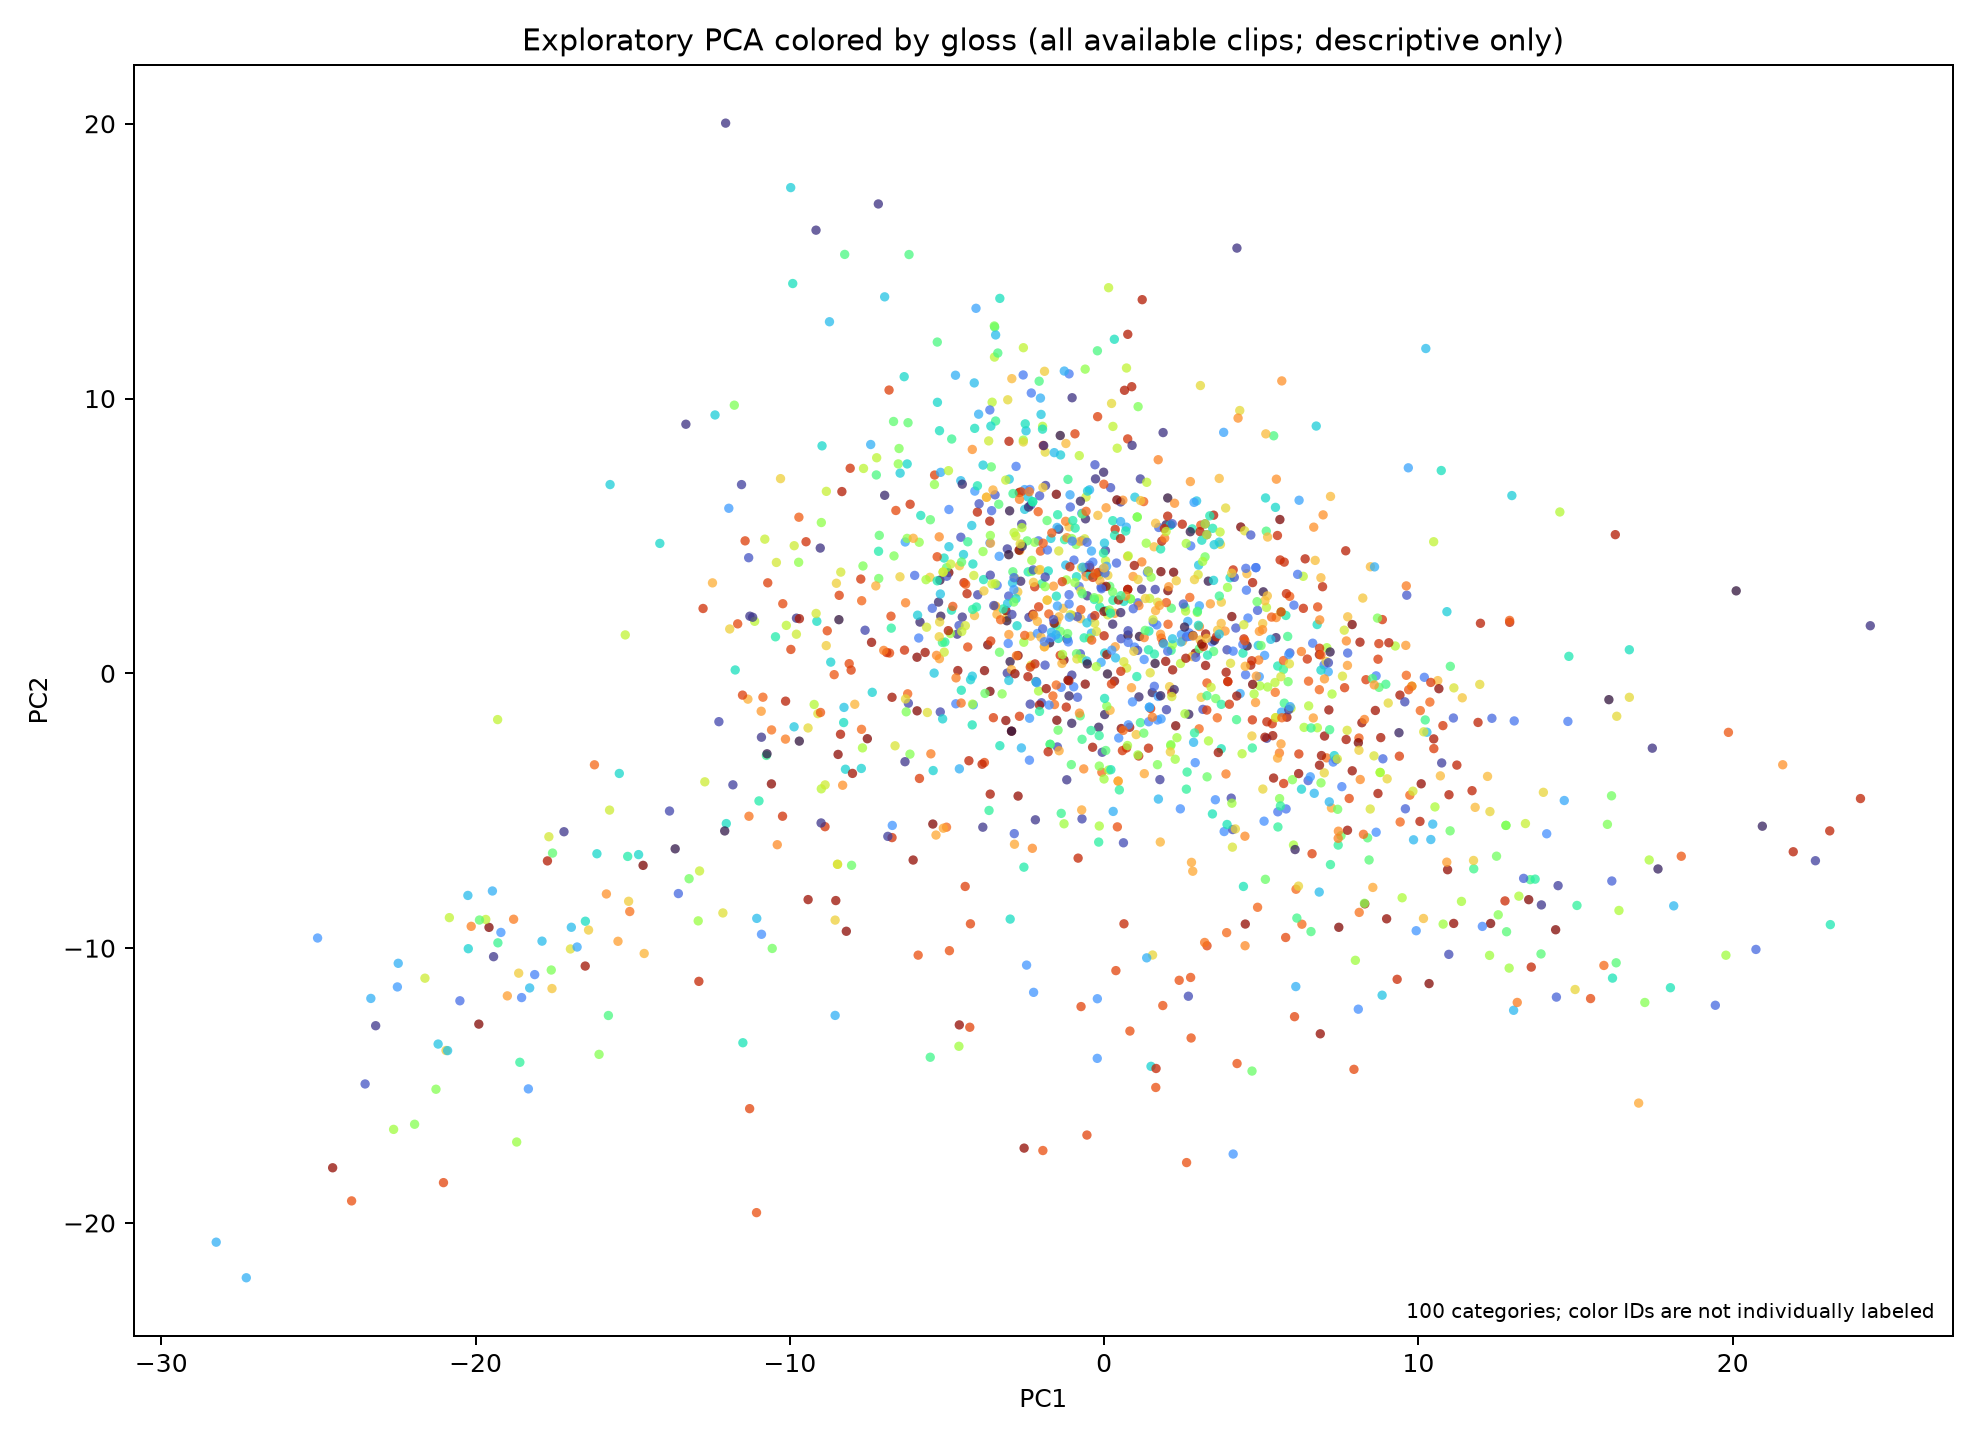
\includegraphics[width=0.82\textwidth]{pca_by_gloss.png}}
\caption{Exploratory PCA view coloured by gloss class.}
\label{fig:pca-gloss}
\end{figure}

\begin{figure}[H]
\centering
\IfFileExists{C:/Users/sarth/sign-language-recognition/sign-language-recognition/report/figures/pca_by_signer.png}{\includegraphics[width=0.82\textwidth]{C:/Users/sarth/sign-language-recognition/sign-language-recognition/report/figures/pca_by_signer.png}}{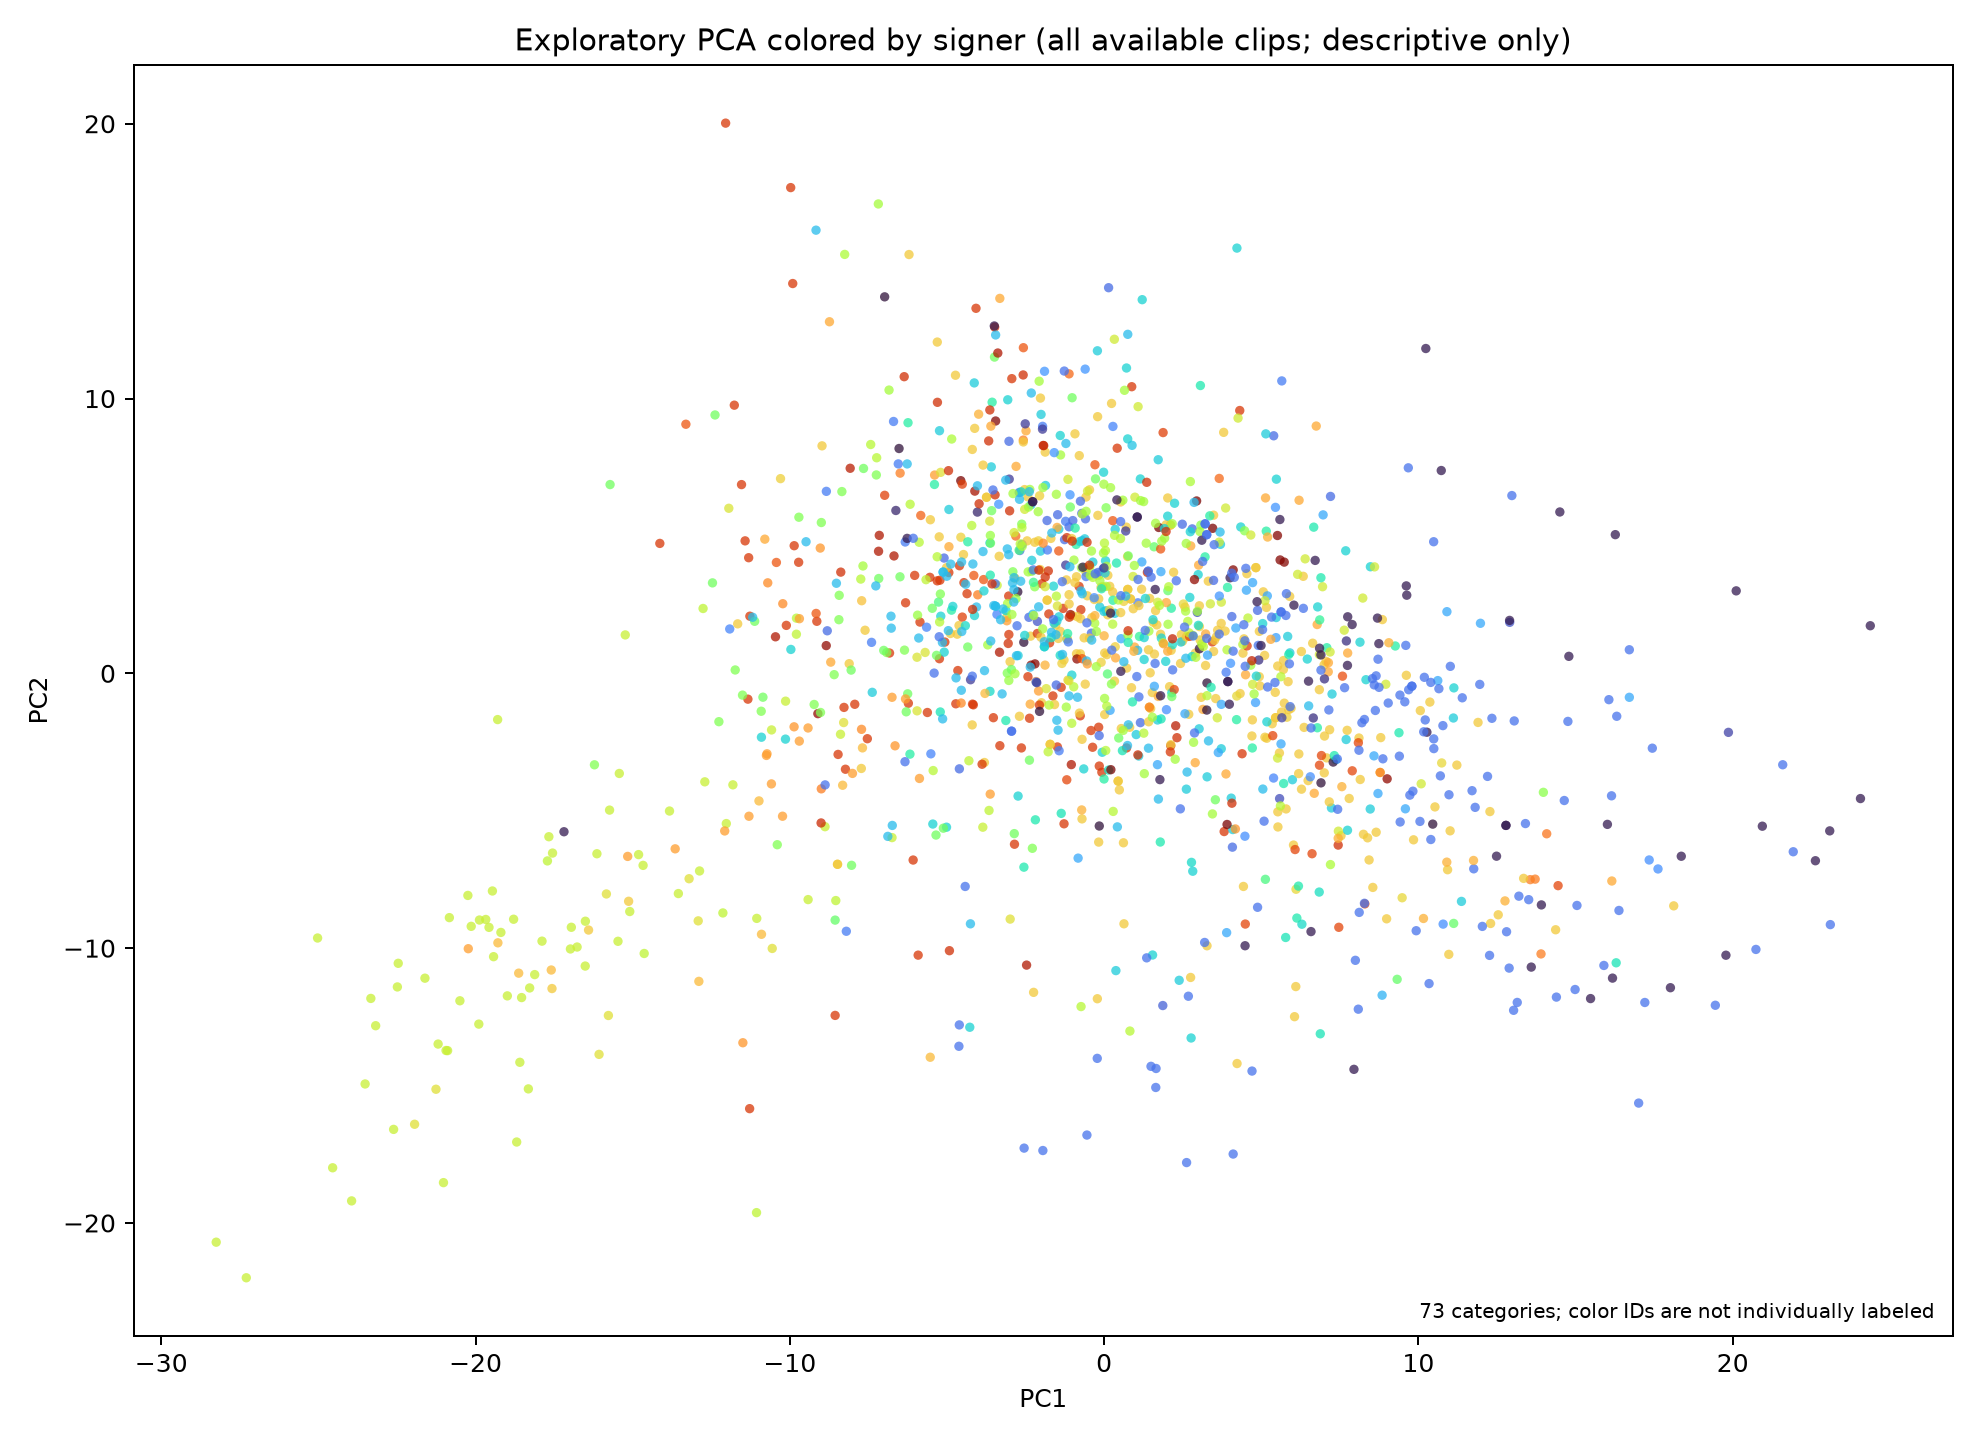
\includegraphics[width=0.82\textwidth]{pca_by_signer.png}}
\caption{Exploratory PCA view coloured by signer.}
\label{fig:pca-signer}
\end{figure}

\section{Model selection protocol}
We chose classical model settings by mean macro-F1 across three signer-grouped folds of the training partition. We then checked each selected setting on validation. For the final score, each model was refit using train plus validation and evaluated once on the frozen test partition. Test results did not guide model or hyperparameter choices. We compared LSTM and GRU input variants with the same grouped-CV approach, then evaluated the selected hand-angle-plus-mask input on the test partition.

The three folds are formed by grouping on signer identity. This means that a fold's validation signers are absent from that fold's training data. Candidate settings are compared on the same fold assignments so differences are not caused by changing the validation examples from one model to another. After selecting a setting, we fit once on the original training partition and record its validation score. For final evaluation, the model is fit again on train plus validation, increasing the number of labelled examples used for the final estimator. Test labels are only used to compute the final metrics.

For the LSTM and GRU, each input variant is evaluated over the same three outer signer-grouped folds. An inner signer-held-out subset of the outer training portion is used to choose the epoch with the best stopping loss. The median best epoch across the outer folds is used when refitting the selected variant. This provides an early-stopping estimate without using the outer validation signers to choose the epoch.

\section{Evaluation measures}
We report accuracy, macro-F1, and balanced accuracy because they answer different questions. Accuracy is the fraction of clips classified correctly:
\[
\mathrm{Accuracy}=\frac{\text{number of correct predictions}}{\text{number of clips}}.
\]
For each gloss, precision measures how many clips predicted as that gloss are correct, while recall measures how many of its true clips are found. The F1 score is the harmonic mean of precision and recall. Macro-F1 computes F1 separately for each class and averages the class scores, giving a rare class the same weight as a common one. Balanced accuracy averages class recall. When support is small, both macro-F1 and balanced accuracy can vary substantially from one clip changing category.

We use grouped-CV macro-F1 to choose classical settings, then report accuracy alongside macro-F1 and balanced accuracy for the final test results. This makes the selection rule explicit and lets readers see whether overall accuracy is hiding weak performance on less frequent glosses. The results from the test split are descriptive of this split; a single test estimate does not provide a confidence interval for new signers.

\section{Compared models}
The classical families are logistic regression, k-nearest neighbours (kNN), RBF support vector machine (SVM), random forest, Extra Trees, and XGBoost. The temporal models are a bidirectional LSTM and a bidirectional GRU with a 96-unit hidden state in each direction and dropout. Class imbalance is addressed with class weighting or sample weighting, depending on the estimator.

The classical search grids were kept modest so that all families could be compared on the same signer-grouped folds. Logistic regression compared $C\in\{0.1,1,10\}$. kNN compared 3, 5, and 9 neighbours with uniform or distance weighting. The RBF SVM compared $C\in\{10,100,300\}$ and a small set of kernel-width choices. Random Forest compared square-root or half-feature sampling and leaf sizes of one or two. Extra Trees compared feature fractions of 0.25, 0.5, and 0.75, leaf sizes of one or two, and balanced or unweighted class settings. XGBoost compared depths two and three with 80 or 140 boosting rounds. These grids are not exhaustive; they are a controlled set of practical candidates for the available training size.

The selected settings are then fixed for validation and test evaluation. The purpose of retuning is to compare each family on its own reasonable configuration, not to make the test score a search target. The saved scripts define the candidate grids and training options, and the per-model result CSVs contain the chosen values.

\chapter{Experiments and Results}
\section{Feature ablations}
Across the grouped training folds, using both hands with hand angles worked better than using coordinates alone or either hand on its own. Adding velocity reduced grouped-CV accuracy in this experiment. Left-hand-only accuracy was lowest; this may reflect both one-handed signs and less reliable left-hand detections. In the sequence-length comparison, the 64-frame Extra Trees representation scored higher than the 16- and 32-frame versions.

The best channel setting reached 41.9\% grouped-CV accuracy and 0.405 macro-F1. Both hands with coordinates alone reached 29.1\%; adding angle information therefore helped in this comparison. The right-hand-plus-angle setting reached 33.2\%, while left-hand-plus-angle reached 17.7\%. This difference should not be read as evidence that the left hand is unimportant to sign language. It is consistent with the missingness measurements: the left hand is missing more often in both video sources, and some WLASL signs are performed primarily with one hand. A model that receives incomplete left-hand measurements has fewer usable features for those clips.

The velocity ablation reached 38.2\%, below the 41.9\% obtained without velocity. Velocity may encode useful motion, but finite differences also magnify frame-to-frame landmark jitter and missingness. With this feature construction and sample size, the extra dimensions did not offset those effects. A different temporal model or a more robust motion representation could behave differently; that question is not answered by this one ablation.

\begin{table}[H]
\centering
\label{tab:ablation}
\begin{tabular}{lr}
\toprule
Feature or setting & Accuracy \\
\midrule
Both hands + angles & 41.9\% \\
Both hands + angles + velocity & 38.2\% \\
Right hand + angles & 33.2\% \\
Both hands, coordinates only & 29.1\% \\
Left hand + angles & 17.7\% \\
16-frame sequences & 41.0\% \\
32-frame sequences & 41.9\% \\
64-frame sequences & 44.2\% \\
\bottomrule
\end{tabular}
\caption{Selected feature and temporal-length ablations (mean signer-grouped CV accuracy).}
\end{table}

We also tested a PCA-plus-logistic-regression baseline on flattened hand and angle sequences. The largest tested component count, 160, reached 19.4\% grouped-CV accuracy and 0.182 macro-F1. Increasing the number of components improved results over the tested range, but PCA did not match the hand-angle Extra Trees representation. Flattening and projecting the full sequence into a linear model removes much of the useful local structure and makes it harder to represent nonlinear class boundaries. This is a diagnostic result for the tested pipeline, rather than a conclusion that dimensionality reduction is always unsuitable.

\begin{table}[H]
\centering
\label{tab:pca}
\begin{tabular}{rrr}
\toprule
PCA components & Grouped-CV accuracy & Macro-F1 \\
\midrule
32 & 14.9\% & 0.137 \\
64 & 16.4\% & 0.153 \\
100 & 18.4\% & 0.174 \\
160 & 19.4\% & 0.182 \\
\bottomrule
\end{tabular}
\caption{PCA component sweep with logistic regression on flattened hand and angle sequences.}
\end{table}

\section{Classical model comparison}
\Cref{tab:classical} compares the six classical models. Extra Trees had the strongest grouped-CV accuracy and the highest test accuracy, 61.8\%. Logistic regression was close on both validation and test. The test score is noticeably higher than the grouped-CV average, so this single split should be read as one estimate; it does not guarantee the same result for new signers.

\begin{table}[H]
\centering
\label{tab:classical}
\small
\resizebox{\textwidth}{!}{%
\begin{tabular}{lrrrrr}
\toprule
Model & CV accuracy & CV macro-F1 & Validation accuracy & Test accuracy & Test macro-F1 \\
\midrule
Extra Trees & 44.2\% & 0.425 & 50.3\% & \textbf{61.8\%} & 0.615 \\
Logistic regression & 42.6\% & 0.414 & 50.3\% & 60.5\% & 0.597 \\
Random forest & 39.4\% & 0.366 & 45.2\% & 55.9\% & 0.548 \\
XGBoost & 35.8\% & 0.331 & 44.6\% & 53.6\% & 0.545 \\
RBF SVM & 34.8\% & 0.341 & 40.5\% & 52.3\% & 0.488 \\
kNN & 27.1\% & 0.260 & 33.3\% & 39.8\% & 0.384 \\
\bottomrule
\end{tabular}
}
\caption{Classical model performance. Cross-validation is three-fold and signer-grouped.}
\end{table}

The grouped-CV columns describe how the selected configuration performed across the three signer-held-out training folds. Validation accuracy uses the fixed 294-clip validation partition. Test accuracy and macro-F1 use the 304-clip test partition after the model settings were selected. The final classical models are refit on 1,162 clips (train plus validation), whereas the grouped-CV models are trained on less data in each fold. This is one reason the test results can be higher than the cross-validation averages. It is not evidence by itself that one split is wrong; the held-out signer groups are different, and the final fit also uses more clips.

\subsection{Selected classical settings}
The grouped-CV search selected an Extra Trees model with balanced class weights, a 0.25 feature fraction, and leaf size one. Logistic regression selected $C=10$. The random forest used square-root feature sampling and leaf size one. The RBF SVM selected $C=100$ and the default scale-based kernel width. XGBoost selected depth two with 140 estimators, while kNN selected five neighbours with distance weighting. These settings are recorded in \texttt{out/comparison.csv} so the reported scores can be tied to the configuration that produced them.

The search criterion was grouped-CV macro-F1, with accuracy used as a tie-breaker. This slightly changes the ranking compared with sorting by the final test accuracy alone. For example, XGBoost has a lower grouped-CV macro-F1 than the RBF SVM but a higher test accuracy in this one split. We retain the model settings chosen before inspecting test metrics and do not re-rank or retune them based on test performance.

\section{LSTM and GRU comparison}
The recurrent models use hand coordinates, hand angles, and a mask for missing values. Their grouped-CV scores were below those of the best classical models. On the one held-out test split, GRU accuracy was 52.0\% and LSTM accuracy was 48.7\%. The gap between grouped-CV and test results is large, which is a reminder that results can vary with the signers in each partition.

\begin{table}[H]
\centering
\label{tab:temporal}
\begin{tabular}{lrrr}
\toprule
Model & Grouped-CV accuracy & Validation accuracy & Test accuracy \\
\midrule
LSTM & 26.4\% & 24.8\% & 48.7\% \\
GRU & 19.6\% & 21.4\% & 52.0\% \\
\bottomrule
\end{tabular}
\caption{Temporal model performance using the selected hand-angle-plus-mask representation.}
\end{table}

Both networks use 96 hidden units in each direction and dropout of 0.35 before the classifier. They are optimized with AdamW, a learning rate of $8\times10^{-4}$, weight decay of $10^{-3}$, batches of 64 clips, and gradient clipping. The LSTM's median best epoch across grouped folds was 40; the GRU's was 32. The input mask gives the model an explicit indicator for which coordinates were observed, instead of forcing it to infer missingness from values filled during normalization.

The temporal models do not lead on grouped CV, despite their ability to model frame order. There are only 868 training examples in total and around 15 clips per class on average, while each recurrent network must estimate many parameters across 100 output classes. The classical models operate on a compact vector and may be less data-hungry in this setting. The results support using recurrent models as part of the comparison, but do not support preferring them for this dataset and feature setup.

\section{Random-split diagnostic}
For comparison, a random clip split averaged 58.8\% across three seeds. It shared 28--32 signers between training and evaluation, so it lets the models see signers they have already encountered. We include it only as a leakage check; it is not a signer-independent result and was not used to choose the final models.

This diagnostic is close to the final test accuracy of the strongest models, but the numbers should not be interpreted as a fair head-to-head comparison. The random split has a different training/evaluation construction and allows familiar signers in both sets. Its role here is to show that the split itself can change what a score means. For the main claim about performance on unseen signers, we rely on the frozen grouped split and grouped-CV results.

\section{Error analysis}
Validation scores hide large differences between glosses. Many classes have only a few clips in the 294-clip validation set, and the Extra Trees model missed every validation example for some classes. Among the most frequent confusions, ``cousin'' was predicted as ``hat'' and ``candy'' as ``pink''. With so few examples per class, these patterns are useful leads, but not firm conclusions.

This error review uses validation predictions, not the held-out test labels. It reports per-class support and recall because a single aggregate value cannot show whether errors are spread evenly across the vocabulary. If a class has one validation clip, a correct prediction changes its recall from zero to one; estimates for these classes are therefore coarse. Confusion pairs also need context: two glosses may share a hand location or movement, but a few errors are not enough to conclude that their signs are intrinsically similar. A larger signer-diverse sample and review of the original clips would be needed to distinguish genuine visual similarity from missed or noisy landmarks.

The examples in the saved analysis include several small confusion pairs rather than one dominant error pattern. This is consistent with a 100-class task in which many glosses have limited support. We use the plots and per-class files to guide inspection, not to claim a complete linguistic account of why two signs are confused.

\chapter{Discussion}
\section{Main findings}
The comparison favoured Extra Trees and logistic regression among the classical models. Using both hands and hand angles was more useful than coordinates alone, and adding velocity did not help in the tested setup. The 64-frame version also did better than shorter sequences in the Extra Trees length comparison.

The gap between grouped-CV averages and final test results needs careful interpretation. The grouped folds use only the training partition and hold out signers within those 868 clips. The final test estimator uses train plus validation, or 1,162 clips, before it predicts the 304 test clips. It therefore has more examples available for fitting than any cross-validation fold. At the same time, the test signers are a particular group of 15 people and the number of clips per class is uneven. Both factors can contribute to a test score higher than the CV average. We report the discrepancy rather than treating the test score as a replacement for the grouped-CV estimate.

The best classical model's test macro-F1 (0.615) is close to its accuracy (0.618), and its balanced accuracy is 0.646. For logistic regression, the corresponding test macro-F1 is 0.597 and balanced accuracy is 0.618. Across the weaker models, the difference between accuracy and macro-F1 is more visible, particularly for kNN. This reinforces the value of looking at more than the fraction of correctly classified clips, while keeping in mind that all these metrics are based on one finite test set.

\section{Limitations}
We could recover clips for 1,466 of the 2,038 metadata instances, and the missing 572 may not be a random subset. There are few examples for many of the 100 glosses, and the data are unevenly distributed across signers. Hand landmarks are often missing or unstable, which removes useful information from the features. We visually checked 20 overlays, but did not manually review every clip. Some frame ranges from YouTube sources may include a few frames of a title card. Finally, the test partition represents only 15 signers, so its score is one estimate and class-level results may change with a different group of signers.

There are also limitations in the feature design. Shoulder normalization helps reduce changes in scale and translation, but it does not correct for all camera-angle or body-proportion differences. The two-bin representation deliberately compresses the sequence and can lose brief movements or fine timing. Joint angles use selected triples rather than a learned skeleton graph, and the simple velocity features can be noisy. Our hyperparameter grids cover a limited set of options, so the winning models are best among the configurations we tested, not necessarily among every possible configuration. Finally, the random-clip diagnostic illustrates leakage but is not a substitute for repeated group-aware evaluations.

\section{Validity and leakage controls}
No signer appears in more than one of the saved train, validation, and test partitions. We selected the classical settings using grouped folds within the training set, and fitted data-dependent preprocessing on the relevant training partition. The random clip experiment is reported separately because its signer overlap makes it unsuitable for the main comparison. We used the test partition after model selection for the scores in this report; it should not be used to choose further settings.

\chapter{Conclusion}
\section{Conclusion}
We assembled a usable landmark set from the available WLASL-100 videos and used it to compare six classical classifiers and two sequence models under a signer-independent split. Extra Trees had the highest test accuracy at 61.8\%; logistic regression followed at 60.5\%. The experiments also exposed practical limits of the data: many videos were unavailable, hand detections were incomplete, and there are few clips per gloss. The final test scores are reported for comparison, but further model choices should be made without using that test set.

\begin{thebibliography}{9}
\addcontentsline{toc}{chapter}{Bibliography}
\bibitem{li2020wlasl}
D. Li, C. Rodriguez, X. Yu, and H. Li, ``Word-level Deep Sign Language Recognition from Video: A New Large-scale Dataset and Methods Comparison,'' in \emph{Proceedings of the IEEE Winter Conference on Applications of Computer Vision}, 2020.

\bibitem{mediapipe_holistic}
Google, ``MediaPipe Holistic,'' MediaPipe documentation. Available at \url{https://ai.google.dev/edge/mediapipe/solutions/vision/holistic_landmarker}.

\bibitem{sklearn}
F. Pedregosa et al., ``Scikit-learn: Machine Learning in Python,'' \emph{Journal of Machine Learning Research}, vol. 12, pp. 2825--2830, 2011.

\bibitem{pytorch}
A. Paszke et al., ``PyTorch: An Imperative Style, High-Performance Deep Learning Library,'' in \emph{Advances in Neural Information Processing Systems}, 2019.

\bibitem{xgboost}
T. Chen and C. Guestrin, ``XGBoost: A Scalable Tree Boosting System,'' in \emph{Proceedings of the 22nd ACM SIGKDD International Conference on Knowledge Discovery and Data Mining}, 2016.
\end{thebibliography}

\chapter*{Project File Workflow}
\addcontentsline{toc}{chapter}{Project File Workflow}
The project files follow the order of the work: define the data, extract landmarks, build features, compare models, and inspect errors. The main files for each stage are:
\begin{enumerate}[leftmargin=*]
  \item \textbf{Dataset definition.} The WLASL-100 metadata and the frozen signer-independent assignments are stored under \texttt{data/processed/WLASL100/}. The split file \texttt{split\_v2.csv} records each clip's gloss, signer, and train/validation/test assignment.
  \item \textbf{Landmark inputs.} MediaPipe arrays are kept in \texttt{landmarks\_repo/} and \texttt{landmarks\_kaggle/}. Each \texttt{.npy} file corresponds to one video. The EDA notebook and \texttt{landmarks\_eda/} outputs summarize coverage, missingness, clip lengths, and signer counts.
  \item \textbf{Preprocessing.} Notebook 05 calls \texttt{scripts/preprocess\_landmarks.py}. It normalizes the coordinates, fills only short gaps, resamples clips, and writes \texttt{preprocessed/sequences\_v1.npz} with the manifest and summary.
  \item \textbf{Feature experiments.} The ablation scripts compare feature channels, PCA sizes, and sequence lengths. They save fold-level results and the 64-frame classical feature matrix under \texttt{ablation\_study/}.
  \item \textbf{Model evaluation.} Notebook 06 runs the classical grouped-CV comparison and final evaluation. Notebook 07 compares LSTM and GRU variants with grouped folds, then evaluates the selected versions. Each model has a \texttt{results.csv} in its folder under \texttt{out/}; \texttt{out/comparison.csv} brings together the six classical models.
  \item \textbf{Error review and report figures.} Notebook 08 summarizes validation errors. The PCA plots and landmark overlay figure are stored in \texttt{report/figures/} for inclusion in this document.
\end{enumerate}
The notebooks are the entry points we use to follow the work, and the Python scripts contain the processing and training steps they run. Saved splits and result files make it possible to trace the reported numbers without rerunning video extraction.

\begin{table}[H]
\centering
\label{tab:file-flow}
\begin{tabularx}{\textwidth}{lX}
\toprule
Stage & Main files and output \\
\midrule
Define the dataset & \texttt{all\_metadata.csv}, \texttt{split\_v2.csv} \\
Store landmarks & \texttt{landmarks\_repo/*.npy}, \texttt{landmarks\_kaggle/*.npy}, and each source's \texttt{index.csv} \\
Inspect data & notebook 01 and \texttt{landmarks\_eda/} \\
Preprocess & notebook 05 and \texttt{preprocessed/sequences\_v1.npz} \\
Compare features and models & notebooks 06--07, scripts in \texttt{scripts/}, and \texttt{out/} \\
Review errors and figures & notebook 08, \texttt{error\_analysis/}, and \texttt{report/figures/} \\
\bottomrule
\end{tabularx}
\caption{How the main project files connect from data preparation to results.}
\end{table}

\appendix
\chapter{Reproducibility Notes}
We used Python 3.12 for this project. Landmark extraction used MediaPipe 0.10.14 and NumPy below version 2 to keep the Holistic API available. The feature and model notebooks use the saved landmark arrays and split, so they can be rerun without processing the original videos again.

The split is fixed in \texttt{data/processed/WLASL100/split\_v2.csv}. Model settings and scores are in the CSV files under \texttt{out/}, and the corresponding run logic is in \texttt{scripts/}. EDA and feature outputs are saved under \texttt{data/processed/WLASL100/}. We set the model seed to 42; the split configuration records the separate search used to select signer groups.

To follow the analysis, start with notebook 01, then use 05 for preprocessing, 06 and 07 for model comparisons, and 08 for validation errors. The acquisition and landmark-extraction notebooks document how we assembled the inputs. The final scripts reuse the selected settings and the same test split; the test results are for final reporting, not another round of tuning.

\end{document}
